\section{Requisitos}

\subsection{Requisitos funcionales}

Los primeros requisitos funcionales del TFG se centraron en la creación de los sistemas y las mecánicas básicas que definen a CoWordle. Después, se fueron detallando funcionalidades más avanzadas.

\begin{itemize}
	\item RF1. Como usuario puedo crear una partida a la que otros jugadores pueden unirse.
	\item RF2. Como usuario puedo unirme a partidas creadas por otros jugadores si poseo el link o el código de la partida.
	\item RF3. Como usuario puedo cambiarme el nombre público en una partida.
	\item RF4. Como usuario puedo ver a todos los jugadores de la partida.
	\item RF5. Como usuario creador de una partida (\textit{host}), tengo el control sobre cuándo quiero que comience ésta.
	\item RF6. Como usuario \textit{host} puedo expulsar a otros jugadores de la partida.
	\item RF7. Como usuario puedo introducir palabras una vez haya comenzado la partida.
	\item RF8. Como usuario puedo ganar si introduzco la palabra objetivo.
	\item RF9. Como usuario puedo conocer cómo de cerca están otros jugadores de la palabra objetivo.
	\item RF10. Como usuario puedo abandonar la partida en cualquier momento y unirme a otras.
	\item RF11. El sistema es capaz de detectar cuándo un jugador se ha unido a la partida, y mostrar al resto de jugadores su nombre.
	\item RF12. El sistema es capaz de detectar cuándo un jugador ha abandonado la partida, y de eliminar su información de ésta. Además, en caso de ser el último jugador, el sistema eliminará la memoria reservada para la partida.
	\item R13. El sistema es capaz de detectar cuándo todos los jugadores han acabado sus intentos, y mostrar una pantalla con la solución y un mensaje indicando que todos los jugadores han perdido.
	\item RF14. Como usuario puedo acceder a la aplicación desde dispositivos móviles, tablets, portátiles y de ordenadores de sobremesa. 
\end{itemize}

\subsection{Requisitos no funcionales}

\begin{itemize}
	\item RNF1. La página web debe ser fácil de usar.
	\item RNF2. Los colores usados en la página web deben ser característicos y reconocibles.
	\item RNF3. El código único de cada partida debe contener pocos caracteres y ser reconocible, para que en caso de que sea transmitido de manera oral, este sea fácil de comunicar.
	\item RNF4. Una vez haya terminado la partida, debe indicarse al los jugadores, quién ha ganado y cuál era la palabra objetivo.
	\item RNF5. Desde la consola de despliegue, se puede atender al avance de la partida, siguiendo los eventos principales que ocurren.
\end{itemize}


\section{Arquitectura general}
El proyecto está dividido en dos repositorios, por un lado está la aplicación web (webapp), que se encarga de realizar la lógica de presentación, así como el \textit{game loop}, y por otro lado tenemos el servidor de backend, donde va toda la lógica de websockets en la parte de servidor.

La comunicación entre aplicaciones se realiza mediante peticiones HTTP y websockets, para ello se utiliza la librería estándar de Javascript proporcionada por el navegador, la librería estándar de Node.js, la librería estándar de Deno y la librería Socket.io.

\begin{figure}[H]
	\centering
	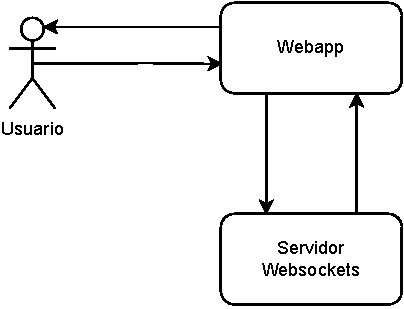
\includegraphics[clip=true,width=0.5\textwidth]{./diagrams/general_arch.pdf}
	\caption{Diagrama de comunicación entre aplicaciones.}
	\label{fig:ex_app_comms}
\end{figure}

El usuario siempre interactúa directamente con la aplicación web, y es esta la que realizará llamadas al servidor.

\begin{figure}[H]
	\centering
	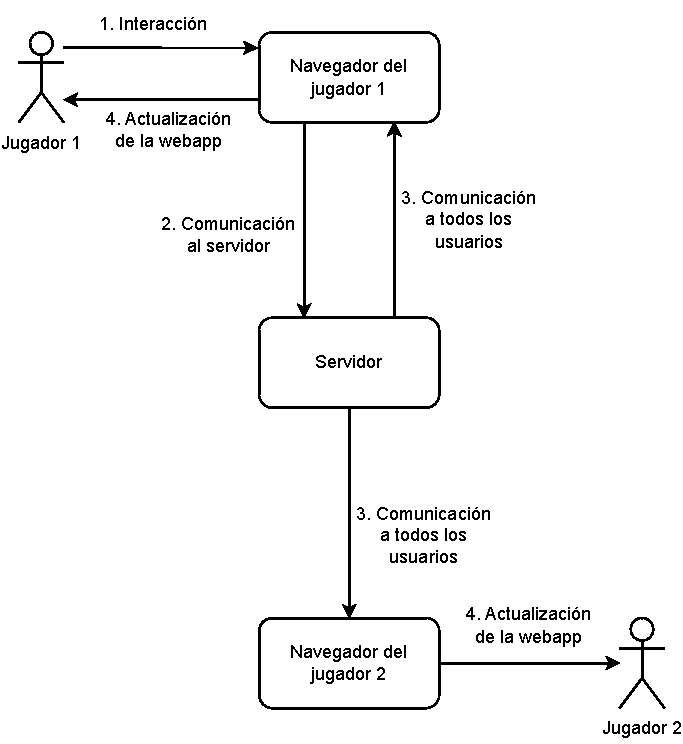
\includegraphics[clip=true,width=0.75\textwidth]{./diagrams/overall_communications.pdf}
	\caption{Diagrama de comunicación a todos los usuarios.}
	\label{fig:ex_comms}
\end{figure}

Al ser una aplicación en tiempo real, es necesario que todos los usuarios estén al tanto de toda la información relevante para la partida. Como se puede ver en la figura \ref{fig:ex_comms}, cada vez que surge una interacción por parte de un usuario, como la inserción de una nueva palabra en el tablero, el servidor es capaz de procesar esta información y enviar a todos los usuarios el resultado relevante para ellos de la acción del otro jugador.


\subsection{Aplicación web}
La aplicación web es la herramienta con la cual el usuario interactúa, permite a este realizar todas las acciones necesarias utilizando un navegador web.

Está desarrollada utilizando SvelteKit para la realización de la lógica, y Tailwind para dar color y estilo.

Como se puede ver en la figura \ref{fig:web_diagram}, el flujo principal que sigue el usuario para poder jugar una partida comienza abriendo la página web de la aplicación web, después, creará o se unirá a una partida ya creada, cuando todos los jugadores estén listos, el creador de la partida le dará al botón de comenzar, y después de una cuenta atrás, a todos los jugadores se les presentará un tablero de Wordle donde pondrán ir escribiendo sus intentos. Si alguno de los jugadores descubre la palabra, todos los jugadores verán una nueva pantalla con el nombre de la persona ganadora, en esta nueva pantalla, los jugadores pueden elegir entre salir de la partida o volver a jugar. En caso de que ningún jugador consiga ganar, se les presentará a todos una pantalla en el que se mostrará la palabra objetivo, y las mismas opciones que en el caso de haber habido un ganador.

\begin{figure}[H]
	\centering
	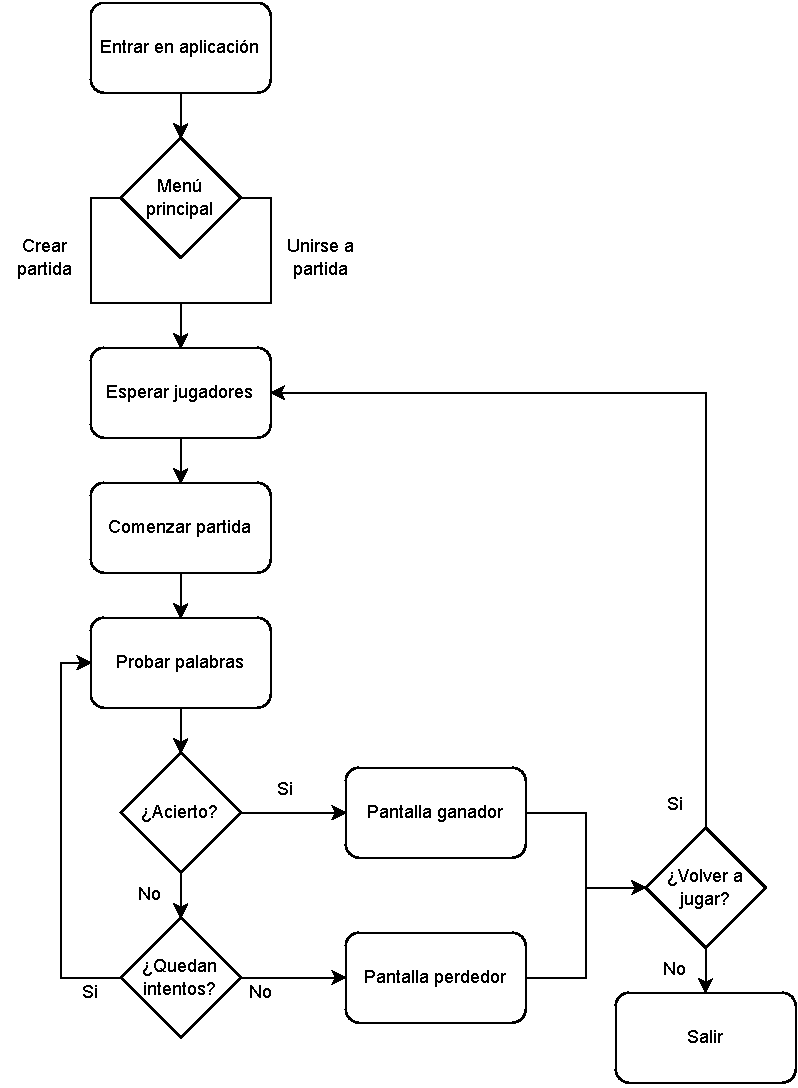
\includegraphics[clip=true,width=0.8\textwidth]{./diagrams/webapp_flow.pdf}
	\caption{Diagrama de flujo de la aplicación web.}
	\label{fig:web_diagram}
\end{figure}

\subsection{Diseño visual}
El diseño visual de la aplicación está inspirado por el diseño original de Wordle tal como se puede ver en la aplicación oficial de Wordle.

En CoWordle se están utilizando diferentes tonalidades para representar los estados de las palabras. Para ver si los colores eran claros y entendibles, se escogió a varios voluntarios que afirman no encontrar mucha diferencia con los significados de los colores oficiales.

\begin{figure}[H]
	\centering
	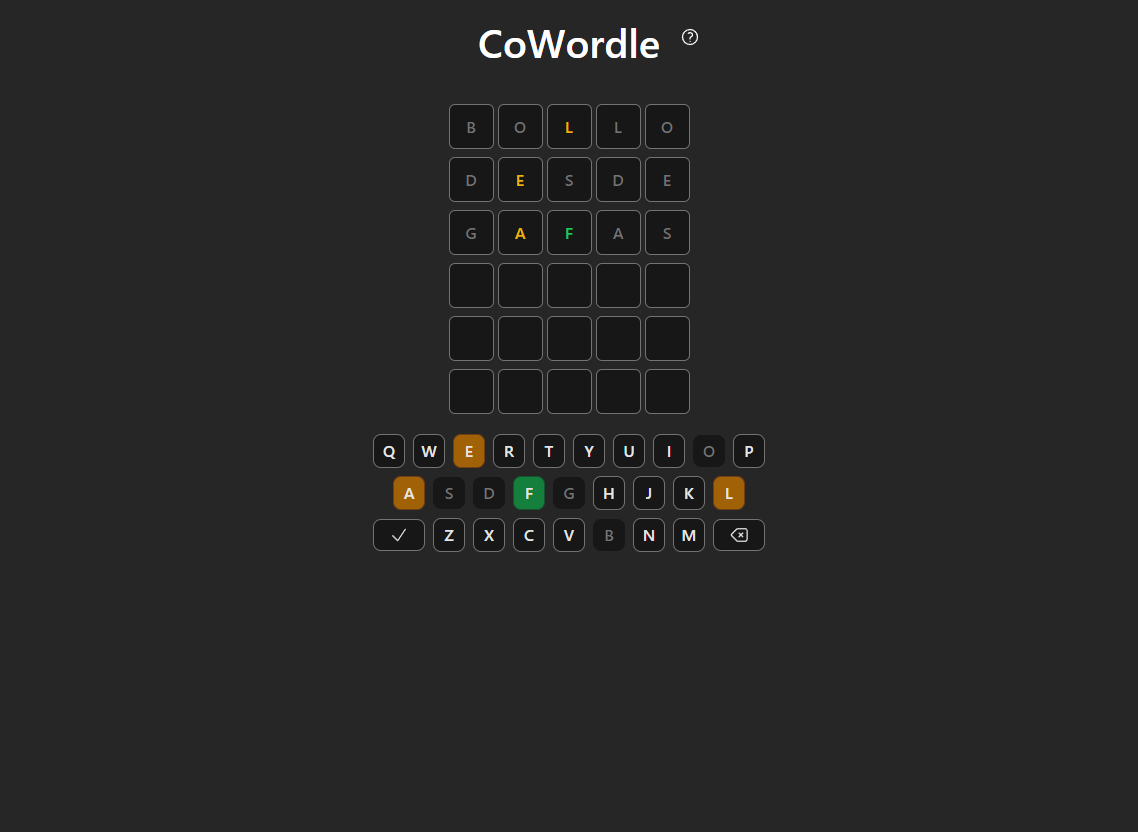
\includegraphics[clip=true,width=\textwidth]{./images/design/cowordle_desktop.png}
	\caption{Aplicación web en vista escritorio.}
	\label{fig:web_desktop}
\end{figure}

Los colores elegidos utilizan tonalidades con colores intensos para poder diferenciarlos con el fondo oscuro. A lo largo de toda la aplicación se reutilizan los mismos colores, creando una sensación de marca.

Los bordes redondeados hacen más amigable la aplicación, y sigue con tendencias modernas que utilizan grandes empresas como Microsoft, por ejemplo, con los bordes de ventana redondeados de Windows 11.

El tablero dispone de un teclado para indicar las letras usadas, oscureciendo aquellas que no se encuentran en la palabra, marcando verde aquellas que se encuentran en la posición correcta y naranjas aquellas que no se encuentran en la posición correcta. El teclado es además completamente funcional.

Toda la aplicación es \textit{responsive}, lo cual significa que es adaptable para cualquier pantalla de cualquier dispositivo, por ejemplo, asi es que como se ve la aplicación en un telefono movil de la compañia Apple.

\begin{figure}[H]
	\centering
	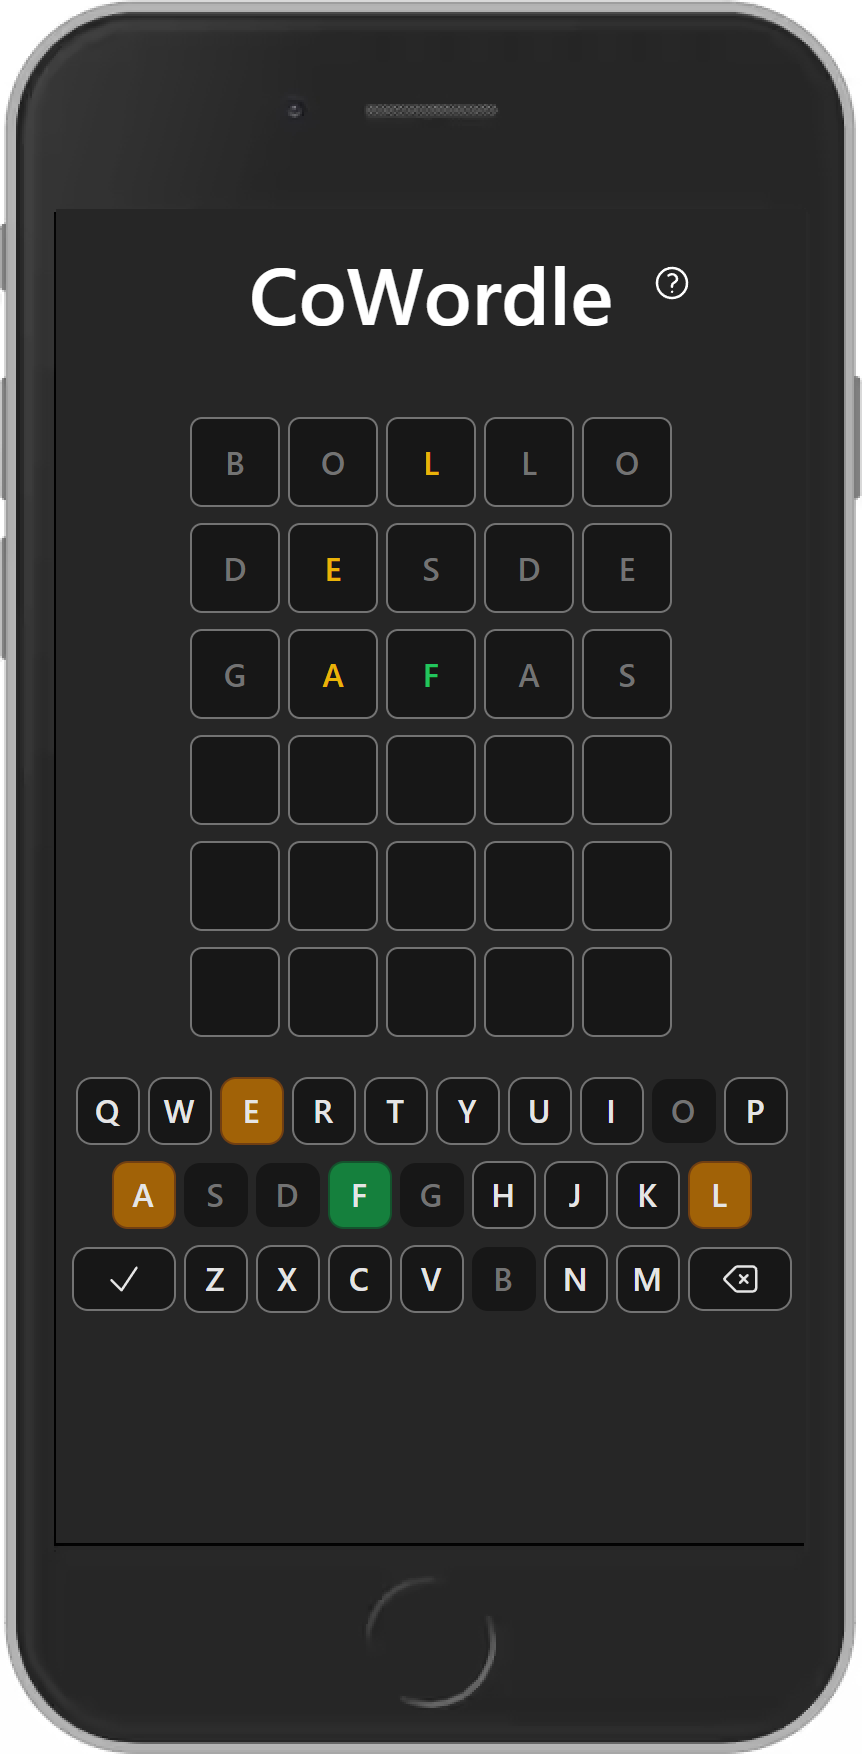
\includegraphics[clip=true,width=0.5\textwidth]{./images/design/cowordle_iphone.png}
	\caption{Aplicación web en un dispositivo móvil.}
	\label{fig:web_iphone}
\end{figure}

Como se puede ver, en lugar del teclado único de cada teléfono móvil, se utiliza el teclado interno de CoWordle, lo cual permite mantener la información que el jugador recibe independientemente del dispositivo.

Además, todas las vistas de la aplicación cuentan con un botón de información que explica brevemente cómo se utiliza la aplicación.


\subsubsection{Comunicación websocket}
\label{sec:ws_comms}
La comunicación websocket ha sido el punto de aprendizaje principal, según se fueron desarrollando las diferentes partes para el trabajo, se fue definiendo lo que acabó siendo una serie de reglas sobre la comunicación diferenciando estas en tres tipos de comunicación diferentes.

Para entender estos tres tipos de comunicación hay que entender primero el sistema de comunicación HTTP. En este tipo de comunicación es el cliente el que inicia la llamada y es el servidor el que responde a esta. Sin embargo, en websockets, el servidor puede enviar información al cliente sin que sea el cliente el iniciador de la llamada. Por ello Websockets funciona por sistemas de eventos, donde el socket puede enviar y esperar comunicación (comunicación bidireccional).

Una vez entendida la comunicación HTTP y la comunicación websocket, y las diferencias entre ambas, va a quedar claro porque en CoWordle se diferencia entre tres tipos distintos de comunicación.

En primer lugar tenemos la comunicación cliente - servidor, donde el cliente envía eventos al servidor, y el servidor puede actuar ante estos eventos, pero no responde a través de ellos. 
Estos eventos se clasifican como eventos OUT, ya que el cliente envía información al exterior. Por ejemplo, la llamada cuando un jugador ha sido expulsado de la partida (\textit{remove\_player}), se envía desde el host de la partida hacia el servidor, cuando el servidor ha procesado este evento, envía a todos los jugadores de la partida el evento \textit{player\_disconnected}, y serán los clientes los que eliminen de sus listados locales al jugador que se ha eliminado.

En segundo lugar tenemos la comunicación servidor - cliente, un ejemplo de esto es el recién descrito \textit{player\_disconnected}, en el que el servidor envía un evento a los jugadores de la sala. Este tipo de eventos se clasifica en CoWordle como IN, porque el cliente recibe información del servidor.

En último lugar el tercer tipo de comunicación se clasifica como DIALOGUE, y se corresponde con comunicación cliente - servidor - cliente, es decir, es el cliente el que comienza la comunicación, el servidor procesa la respuesta y se la envía al cliente con el mismo nombre de evento con el que la llamada había comenzado, hasta que la llamada no ha sido respondida, el cliente se quedará esperando una respuesta de manera asíncrona, es decir, sin bloquear al resto de la aplicación.

\subsection{Servidor Websockets}
El servidor de websockets está implementado utilizando Deno y una librería que ayuda al manejo de eventos para los websockets llamada Socket.io. Deno se utiliza para levantar el servidor y para recibir peticiones HTTP, existe un endpoint necesario para que Socket.io cree la conexión de Websockets, y uno más para la creación de la partida. 

\subsubsection{Sistema de eventos}
El servidor responde a peticiones HTTP y de Websockets creando eventos que son respondidos de manera secuencial por funciones lambda, cada función sólo responde a un evento, devolviendo una respuesta.
Javascript es una tecnología uni-hilo, pero es capaz de realizar concurrencia utilizando primitivas asíncronas llamadas promesas, cuando una función marcada como asíncrona se ejecuta, el motor de Javascript la guarda como evento, este evento será manejado cuando el motor de Javascript lo considere oportuno. Por ejemplo, cuando la CPU está esperando una lectura de la memoría, Javascript puede cambiar el contexto y procesar otras funciones. De está manera, Javascript es capaz de maximizar la utilización de su hilo de ejecución.

\subsubsection{Eventos disponibles}
El servidor permite la comunicación cliente-servidor utilizando las siguientes rutas HTTP:

\tutor{qué distingue estos eventos de llamadas HTTP como los que se muestran más abajo?}
\alumno{No acabo de ver como solucionar esto, he llamado 'eventos' a las rutas de WebSockets, y he dejado las 'normales' como rutas HTTP, pero no se que más puedo hacer para solucionarlo}
\begin{itemize}
	\item \textit{/create-route}, genera un nuevo identificador de partida. Este identificador es fundamental para la comunicación entre el cliente y el servidor ya que permite la identificación de la partida para realizar las operaciones necesarias.
	\item \textit{/testing/solution}, este endpoint está disponible para poder realizar un tests de integración de flujo completo.
\end{itemize}

A parte de las rutas HTTP, el servidor permite la comunicación WebSocket utilizando los siguientes eventos:

\begin{itemize}
	\item \textit{setup} es un evento de tipo diálogo que une a un jugador a la partida, es necesario enviar como parámetros el código de la sala generado por /create-room y el nombre del usuario que se va a unir a la partida, este evento avisa a todos los demás jugadores de la sala que se ha unido el jugador emitiendo el evento \textit{player\_connection}.
	\item \textit{update\_player\_name} es un evento de tipo diálogo que permite a los jugadores actualizar su nombre, especialmente útil porque el primer nombre que recibe cada jugador al conectarse a la partida es aleatorio entre una combinación de posibilidades.
	\item \textit{remove\_player} es un evento de tipo out que solo pueden utilizar el creador de la partida, y permite expulsar a jugadores de la partida. Cuando ha expulsado a un jugador emite un evento \textit{player\_disconnected} que notifica al resto de usuarios de la desconexión.
	\item \textit{validate\_word} es un evento de tipo diálogo que comprueba un intento de un jugador con la palabra objetivo. El resultado de la operación de comprobación es un array de una enumeración (\textit{WordlePoints}) que indican el resultado de cada letra en la palabra (si no se encuentra en la palabra, si se encuentra en la palabra, si está en la posición correcta). Este resultado se envía directamente al jugador que ha ejecutado el evento, pero también se envía a los demás jugadores para indicar en el scoreboard el conocimiento de cada jugador. Además, se comprueba si la partida ha terminado por que el intento coincide con la palabra objetivo, y si todos los jugadores han perdido porque se han quedado sin intentos.
	\item \textit{start\_game} es un evento de tipo out que permite al host de la partida empezar. En el momento que se lanza este evento todos los jugadores reciben el evento \textit{start\_prematch} que les indica cuándo comenzará la partida.
	\item \textit{disconnect} es un evento nativo de Socket.io, que permite al servidor conocer cuando un jugador se ha desconectado de la partida, existen varias razones para que se ejecute este evento, por ejemplo, que el jugador haya perdido la conexión con internet, o que el jugador haya decidido abandonar la partida cerrando el navegador. En este evento se comunica al resto de jugadores que este ha abandonado la partida, en caso de ser el jugador que ha creado la partida el que la abandona, se cierra también para el resto de jugadores.
\end{itemize}


\subsubsection{Endpoints HTTP}
Como el objetivo del trabajo era el aprendizaje de la comunicación bidireccional, la mayor parte de la comunicación se realiza a traves de websockets, aun asi existen dos rutas disponibles para la realización de comunicación HTTP:

\begin{itemize}
	\item \textit{/create-room} crea una nueva partida para que los jugadores puedan unirse y jugar. Cada partida está identificada por un identificador que se genera durante este proceso.
	\item Existe también una ruta reservada por la librería de Socket.IO que se utiliza internamente para establecer la conexión websocket. Esta ruta está completamente manejada por Socket.IO.
\end{itemize}

\subsubsection{Identificador de partida}
Cada partida tiene un identificador único de seis cifras generado pseudo-aleatoriamente llamado roomCode. El roomCode lo generará el servidor tras la petición HTTP. Esta ruta únicamente reserva el código generado para la partida, utilizando ese código los jugadores son capaces de unirse a la partida inicialmente, el código también se utiliza para realizar la comunicación cliente-servidor.


\section{Diseño e Implementación}

\subsection{La reutilización de componentes}
Svelte, la tecnología que he usado para hacer los componentes de front, se basa en la creación de componentes que puedan ser reutilizados en diferentes situaciones, la reutilización de código se considera buena práctica en todo el ámbito de la ingeniería informática. Por ello parece importante destacar que una buena elección de la tecnologías es solo la base, y es necesario hacer un buen uso de estas para poder llegar a un buen resultado, por ello en este apartado quiero destacar un buen uso de componentes de Svelte.

Existe un componente que se reutiliza varias veces a lo largo de la aplicación, el componente llamado \textit{$<$Word$>$}, que se encuentra en el archivo \textit{Word.svelte} de la aplicación cowordle-webapp.

Este componente se utiliza como botones estilizados en el menú principal, en este primer uso, el componente muestra la palabra elegida por el desarrollador, indicando al usuario que es un botón con el que puede interaccionar.

\begin{figure}[H]
	\centering
	
\includegraphics[clip=true]{images/reusing/host_component.png}
	\caption{Imagen del componente como botón.}
	\label{fig:comp_host_image}
\end{figure}

Después, se vuelve utilizar como huecos para las palabras mientras se juega, en este caso la palabra tiene distinto número de huecos disponibles, además está completamente vacía de texto.

\begin{figure}[H]
	\centering
	
\includegraphics[clip=true, width=0.75\textwidth]{images/reusing/empty_component.png}
	\caption{Imagen del componente con texto vacio.}
	\label{fig:comp_empty}
\end{figure}


Cuando el jugador interacciona con el teclado mientras juega, las palabras se van llenando de letras.

\begin{figure}[H]
	\centering
	
\includegraphics[clip=true, width=0.75\textwidth]{images/reusing/filled_component.png}
	\caption{Imagen del componente con texto.}
	\label{fig:comp_filled}
\end{figure}

Además, las letras muestran el progreso de la palabra objetivo, utilizando los colores característicos.

\begin{figure}[H]
	\centering
	
\includegraphics[clip=true, width=0.75\textwidth]{images/reusing/colored_component.png}
	\caption{Imagen del componente con texto y colores.}
	\label{fig:comp_colored}
\end{figure}

Todas las imágenes mostradas representan el mismo componente de Svelte, y permiten mostrar las ventajas de utilizar tecnologías web reactivas.
Comenzando por el principio, necesitamos un componente que sea capaz de mostrar texto.

\begin{figure}[H]
	\centering
	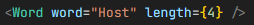
\includegraphics[clip=true, width=0.6\textwidth]{images/reusing/code_simple_component.png}
	\caption{Imagen código para utilizar el componente.}
	\label{fig:comp_simple_code}
\end{figure}

Así es como se utiliza el componente \textit{$<$Word$>$}, para mostrar el texto de la primera imagen simplemente es necesario definir la palabra a mostrar y su longitud.

También queremos que el componente reciba texto del usuario dinámicamente, esto sería posible reprogramando al componente o creando uno nuevo, pero realmente ya tenemos esta funcionalidad sin necesidad de programar nada más. En lugar de utilizar como argumento para el parámetro word un string fijo, podemos utilizar una variable, e indicarle a Svelte que esa variable es reactiva utilizando, la directiva bind, que recalcula el componente cada vez que cambia el contenido de la variable pasada.

\begin{figure}[H]
	\centering
	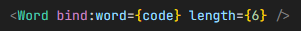
\includegraphics[clip=true, width=0.75\textwidth]{images/reusing/code_dyn_component.png}
	\caption{Imagen código para utilizar el componente con texto dinámico.}
	\label{fig:comp_dyn_code}
\end{figure}

En este caso estamos utilizando la directiva \textit{bind} para hacer que el componente se redibuje cada vez que cambia la variable code. Esto significa que nuestro componente es ajeno al texto que presentamos, y es responsabilidad de otros componentes seleccionar el texto a mostrar.

Parece un pequeño detalle, pero esta flexibilidad de desarrollo simplifica el código haciéndolo muy reutilizable y componible.

La primera implementación del componente \textit{$<$Word$>$} se hizo cuando se comenzó el proyecto,  y sin mucho cambio, ha llegado a utilizarse en otras partes de la aplicación en las que no se había llegado a pensar cuando se creó el componente, y eso demuestra que se realizó un buen diseño inicialmente.

\subsection{Tipados en la comunicación websocket}
Como se ha explicado en el apartado \ref{sec:ws_comms}, la comunicación websocket con el servidor de CoWordle se clasifica en tres grupos, según sea cliente - servidor, servidor - cliente y cliente - servidor - cliente. En este apartado se va a explicar cómo de fácil es realizar esta comunicación independientemente del tipo de esta.

Toda esta capa de tipado se construye como un wrapper sobre el socket expuesto por Socket.IO. Esto permite utilizar la potencia de Socket.IO, mientras se provee la seguridad de tipos y la comodidad del auto-completado del IDE, además permite la utilización de distintos métodos del wrapper según el tipo de comunicación que vayamos a realizar, siendo estos: \textit{emit} para los eventos cliente-servidor, \textit{on} para los eventos servidor-cliente, y \textit{dialogue} para los eventos cliente-servidor-cliente.


\subsubsection{Comunicación IN}
Para la comunicación IN, es el servidor quien envía el evento al cliente, por ello el cliente debe quedarse esperando a que el servidor envíe la petición.

El wrapper expone un método \textit{on}, que permite añadir un callback cuando el evento sea emitido, es decir, cuando el servidor lo emite y el cliente lo haya recibido.

\begin{mytypescript}[float={!h},caption={Uso de eventos websocket IN.},label={alg:ws_in_usage}]
	this.socket.on("player_connected", ({ newPlayer }) => {
		this.addPlayer(newPlayer);
																								
		this.notifies.playersUpdated.broadcast(this.players);
	}); 
\end{mytypescript}

En el framento del Código \ref{alg:ws_in_usage} se puede observar cómo se está definiendo que cuando el evento \textit{player\_connected} ocurra, la función lambda debe ejecutarse. El evento \textit{player\_connected} está declarado utilizando tipos de la siguiente manera (fragmento de Código \ref{alg:player_connected_type}).

\begin{mytypescript}[float={!h},caption={Ejemplo de declaración de la comunicación IN.},label={alg:player_connected_type}]
	export type WebsocketInEvent = {
		...
		player_connected: {
			newPlayer: InitialPlayerInfoDto;
		};
		...
	};
\end{mytypescript}

En esta declaración tan solo necesitamos indicar los parámetros que nos van a llegar del servidor, esta declaración de tipos permite dos mejoras con respecto a los eventos directos de Socket.IO. Por un lado, el IDE ofrece ayuda sobre los nombres de los eventos disponibles sobre los que hacer la espera, además, nos ofrecerá ayuda sobre los parámetros que vamos a recibir según el nombre que indicamos en el primer argumento.

Todo esto es posible gracias al poderoso sistema de genéricos proporcionado por Typescript.

\begin{mytypescript}[float={!h},caption={Declaración del método \textit{on}.},label={alg:on_method}]
	on<TEvent extends EventName<WebsocketInEvent>, TArgs extends WebsocketInEvent[TEvent]>(
	event: TEvent,
	callback: (args: TArgs) => void,
	): void {
		this.socket.on(event as string, callback);
	}
\end{mytypescript}

Como se puede ver en la definición del método \textit{on} (fragmento de Código \ref{alg:on_method}), el primer parámetro es el nombre del evento, que está tipado como el genérico \textit{TEvent} que está a su vez definido como un nombre de evento de la lista de eventos IN. El segundo parámetro es el callback a que se llamará cuando el evento se ejecute, este parámetro está tipado como una función que recibe un argumento del tipo \textit{TArgs}, que es de la lista de eventos IN, aquel que coincide con la el genérico \textit{TEvent}. Todo ello ofrece suficiente información al IDE para ser capaz de autocompletar todo lo necesario para que el programador esté seguro de lo que está programando es correcto, y además, mejora la mantenibilidad a largo plazo, porque en caso de cambiar el tipado de algún evento IN de la lista de eventos, el cambio sería reflejado automáticamente en toda la aplicación y en caso de que no coincidieran los nuevos tipos con los antiguos, Typescript indicaría al programador donde ha ocurrido el fallo de tipado.

\subsubsection{Comunicación OUT}
La comunicación OUT es aquella que ocurre en dirección cliente - servidor, el cliente solo pretende comunicar información al servidor, sin esperar nada de respuesta.

\begin{mytypescript}[float={!h},caption={Ejemplo de uso del método \textit{emit}.},label={alg:emit_usage}]
	startGame(wordListId: string): void {
		this.socket.emit("start_game", {
			wordListId,
		});
	}
\end{mytypescript}

En el ejemplo \ref{alg:emit_usage} se puede ver cómo se emite un evento al servidor, para emitir un evento necesitamos el nombre del evento a emitir, y necesitamos también la información que queremos enviar por el socket.

Al igual que la comunicación IN, el sistema dispone de un lugar donde definir todos los eventos OUT, para el ejemplo mostrado en la figura anterior, el evento está definido como se ve en el fragmento de Código \ref{alg:start_game_type}.

\begin{mytypescript}[float={!h},caption={Ejemplo de declaración de la comunicación OUT.},label={alg:start_game_type}]
	export type WebsocketOutEvent = {
		...
		start_game: {
			wordListId: string;
		};
	};
\end{mytypescript}

Esta definición es la versión inversa de la mostrada en los eventos IN, lo que declaramos dentro del evento representan los argumentos que vamos a enviar al servidor, mientras que la comunicación IN se definen los argumentos que íbamos a recibir. A pesar de la diferencia de uso, la forma de declarar ambos es la misma.

% vs-code
\begin{mytypescript}[float={!h},caption={Declaración del método \textit{emit}.},label={alg:emit_method}]
	emit<TEvent extends EventName<WebsocketOutEvent>,TArgs extends WebsocketOutEvent[TEvent]>(
	event: TEvent,
	args: TArgs,
	): void {
		this.socket.emit(event, args);
	}
\end{mytypescript}

Si nos adentramos en la declaración del método \textit{Emit} (fragmento de Código \ref{alg:emit_method}), que como ya hemos visto es el que se utiliza para la comunicación OUT, volvemos a ver la aparición de un tipo genérico \textit{TEvent}, con la diferencia de que este \textit{TEvent} es un evento de la lista de eventos OUT, la otra diferencia con el método \textit{on}, es que en este utilizamos el argumento \textit{args} como el argumento del método \textit{emit} de Socket.IO, que es el que realizara la petición siguiendo el estándar websocket.

El método \textit{emit} ofrece al programador la misma seguridad y mantenibilidad que el método \textit{on}, además, su similitud de uso, ayuda a que sea más fácil usarlo por programadores de todos los niveles.

\subsubsection{Comunicación Dialogue}
En la comunicación de tipo Dialogue, el cliente envía un evento al servidor, esperando una respuesta de vuelta. Este tipo de comunicación es más compleja de implementar que las otras, pero su uso en CoWordle sigue siendo muy simple.

\begin{mytypescript}[float={!t},caption={Ejemplo de uso del método \textit{dialogue}.},label={alg:dialogue_example}]
	const { localPlayer, players, hostPlayer } = await this.socket.dialogue("setup", {
		playerName: this.localPlayer.name,
		roomCode: this.roomCode,
	});
\end{mytypescript}

Como se puede ver en el ejemplo \ref{alg:dialogue_example}, para usar un evento de tipo Dialogue tan solo tenemos que llamar al método \textit{dialogue} del wrapper. Aunque el tipo Dialogue es muy similar a lo que es una petición HTTP al uso, usando el evento permitimos que toda la comunicación del mismo tipo (comunicación en tiempo real sobre el juego) se realice utilizando un único canal de comunicación, además, nos permite utilizar la información guardada en el socket desde el servidor.

El primer argumento define el evento que vamos a emitir y sobre el que vamos a esperar la respuesta. El segundo argumento describe los datos que vamos a enviar. Como respuesta obtendremos una \textit{promesa} de la respuesta que recibiremos del servidor cuando este responda.

Para declarar un evento del tipo Dialogue, se utiliza una sintaxis muy cómoda, que permite diferenciar en un solo vistazo los tipos que vamos a enviar y los tipos que vamos a recibir (fragmento de Código \ref{alg:dialogue_usage}).

\begin{mytypescript}[float={!t},caption={Ejemplo de declaración del tipo de evento Dialogue.},label={alg:dialogue_usage}]
	export type WebSocketDialogueEvent = {
		...
		setup: (args: { roomCode: string; playerName: string }) => {
			players: InitialPlayerInfoDto[];
			hostPlayer: InitialPlayerInfoDto;
			localPlayer: InitialPlayerInfoDto;
			roomState: RoomState;
		};
		...
	};
\end{mytypescript}

El evento se declara como una función donde los argumentos son los datos a enviar a servidor, y cuya respuesta son los tipos que vamos a recibir del servidor.

Como explicaba anteriormente, la implementación es un poco más compleja que en los tipos de comunicación anteriores, como se ve en el fragmento de Código \ref{alg:dialogue_method}. El primer parámetro coincide con los de los otros tipos de comunicación, volviendo a usar el \textit{TEvent}. El segundo argumento extrae los parámetros de la función declarada como evento. El valor de retorno del método se define como una \textit{promesa} del valor de retorno definido en función del evento.

Con esta implementación estamos manteniendo la sencillez de uso que teníamos con los otros tipos de comunicación, pero estamos creando una comunicación más clásica, donde el cliente y el servidor se comunican como si fuera una petición HTTP normal.

\begin{mytypescript}[float={!t},caption={Implementación del método \textit{dialogue}.},label={alg:dialogue_method}]
	async dialogue<TEvent extends EventName<WebSocketDialogueEvent>, TEventMethod extends WebSocketDialogueEvent[TEvent]>(
	event: TEvent,
	params: Parameters<TEventMethod>[0],
	eventResponse?: string
	): Promise<ReturnType<WebSocketDialogueEvent[TEvent]>> {
		return new Promise((resolve, reject) => {
			this.socket.emit(event, params);

			this.socket.on<string>(eventResponse || event, (result) => {
				this.socket.off(event);
				resolve(result);
			});

			setTimeout(() => reject("timeout"), 10000);
		});
	}
\end{mytypescript}


\section{Pruebas}

Como el proyecto está dividido en dos repositorios distintos con tecnologias distintas, es necesario explicar como se han realizado los tests en ambos repositorios.

\subsection{Webapp}
Para la webapp se han realizado pruebas unitarias de componentes, para ello se ha utilizado Playwright. Como se ha explicado en la sección de tecnologías, Playwright es la librería recomendada para el testeo de componentes.

Playwright utiliza un navegador \textit{headless} internamente para comprobar que los componentes están funcionando. Además, permite seleccionar qué tecnología de navegador se quiere probar. Para CoWordle se realizan tests en todas las tecnologías principales, Firefox, Chromium y Webkit.

Los tests realizados incluyen comprobaciones para ver si los componentes son montados correctamente en la pantalla, si los componentes muestran los textos correctamente y si los colores, especialmente en los colores de juego, se muestran correctamente.

Un ejemplo de test donde se ha comprobado si el componente se monta correctamente, se puede observar en el archivo \textit{tests/components/word.test.ts}. En este test se puede comprobar que primero se monta el componente con los props necesarios, y después se realiza la comprobación de que el componente sea visible.

\begin{mytypescript}[float={!h},caption={Ejemplo test visibilidad componente.},label={alg:test_visibility}]
	test("component is displayed correctly", async ({ mount }) => {
		const comp = await mount(Word, {
			props: {
				word: "Hello",
				length: "Hello".length,
			},
		});

		await expect(comp).toBeVisible();
	});
\end{mytypescript}

Un ejemplo de test donde se comprueba el contenido textual de un componente se puede ver en el mismo archivo que el test anterior.
En este test (fragmento de Código \ref{alg:test_text}) se puede comprobar cómo se monta el componente y se prueba que el texto interno del componente coincide con lo esperado.

\begin{mytypescript}[float={!h},caption={Ejemplo test con texto.},label={alg:test_text}]
	test("contents are displayed correctly", async ({ mount }) => {
		const comp = await mount(Word, {
			props: {
				word: "Hello",
				length: "Hello".length,
			},
		});


		await expect(comp).toContainText("Hello");
	});
\end{mytypescript}

Un ejemplo de test donde se comprueba que los colores de las letras se puede volver a ver en el archivo ya visto (fragmento de Código \ref{alg:test_colors}).

\begin{mytypescript}[float={!h},caption={Ejemplo test colores.},label={alg:test_colors}]
	test("colors are shown correctly", async ({ mount }) => {
		const word = "SUN";


		const comp = await mount(Word, {
			props: {
				word,
				length: word.length,
				results: [WordlePoints.Exact, WordlePoints.InWord, WordlePoints.Missing]
			},
		});


		const innerLetters = await comp.getByRole("paragraph").all();


		await expect(innerLetters[0]).toHaveClass(/letter-exact/);
		await expect(innerLetters[1]).toHaveClass(/letter-in-word/);
		await expect(innerLetters[2]).toHaveClass(/letter-missing/);
	});
\end{mytypescript}

En este ejemplo se monta el componente, con las letras a mostrar y los resultados que deberían de mostrar los colores de las letras CoWordle. Una vez montado el componente, se extraen todas las letras de este, y se comprueba que cada letra tenga la clase HTML correcta. Se comprueban las clases HTML porque internamente a cada clase HTML le corresponde un color CSS. Si en algún momento se decidiera cambiar los colores, no habría que modificar los tests, ya que en ningún momento se comprueban colores concretos.

Para poder ejecutar los tests en local, es necesario utilizar el comando \ref{alg:execute_test_playwright}.

\begin{mypython}[float={!t},caption={Comando para ejecutar los tests de Playwright},label={alg:execute_test_playwright}]
	$ npm run test-ct
\end{mypython}

Una vez ejecutado el comando, Playwright comenzará a realizar los tests, una vez haya terminado nos abrirá una página web donde mostrarán los resultados.

\begin{figure}[H]
	\centering
	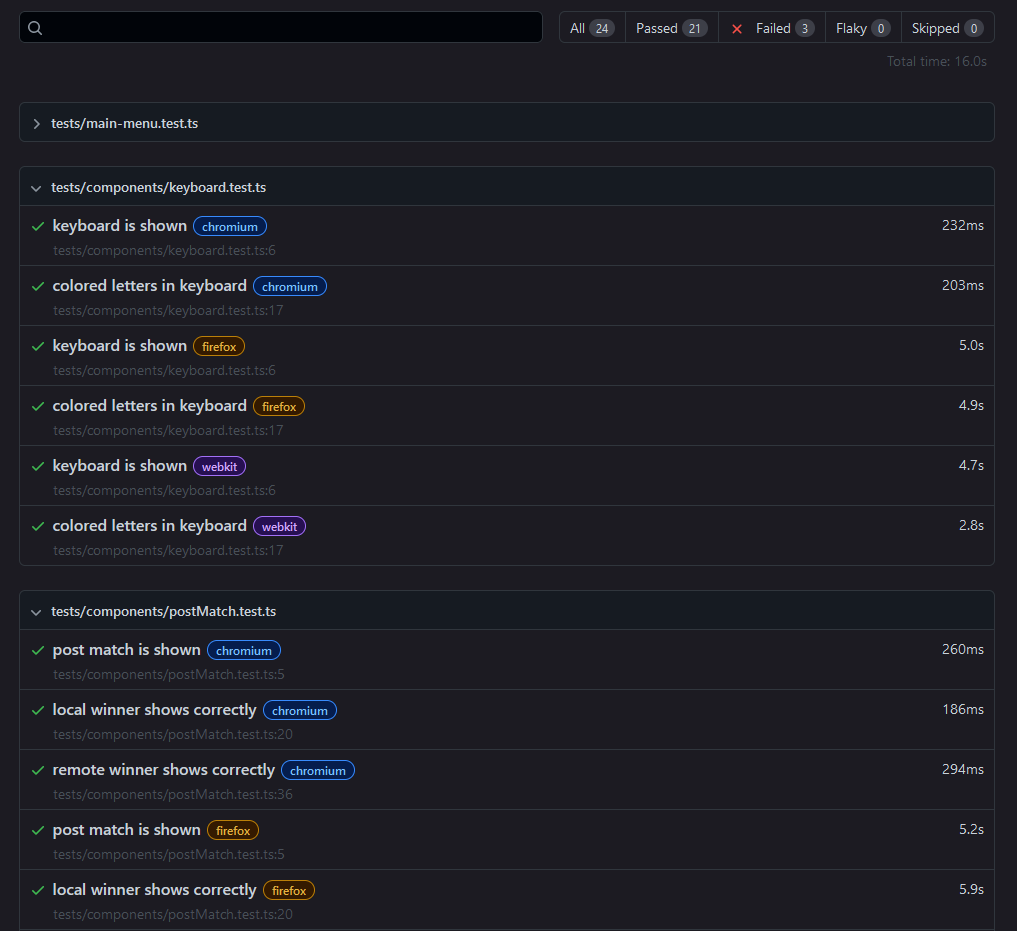
\includegraphics[clip=true, width=\textwidth]{images/tests/playwright_web.png}
	\caption{Imagen resultado de realizar los tests.}
	\label{fig:playwright_tests_result}
\end{figure}

En la página mostrada en la Figura \ref{fig:playwright_tests_result} podemos inspeccionar cada test realizado, pudiendo ver las comprobaciones que se han realizado en cada uno, como se puede ver en la Figura \ref{fig:playwright_test_result}, y en caso de haber fallado, la razón del error.

\begin{figure}[H]
	\centering
	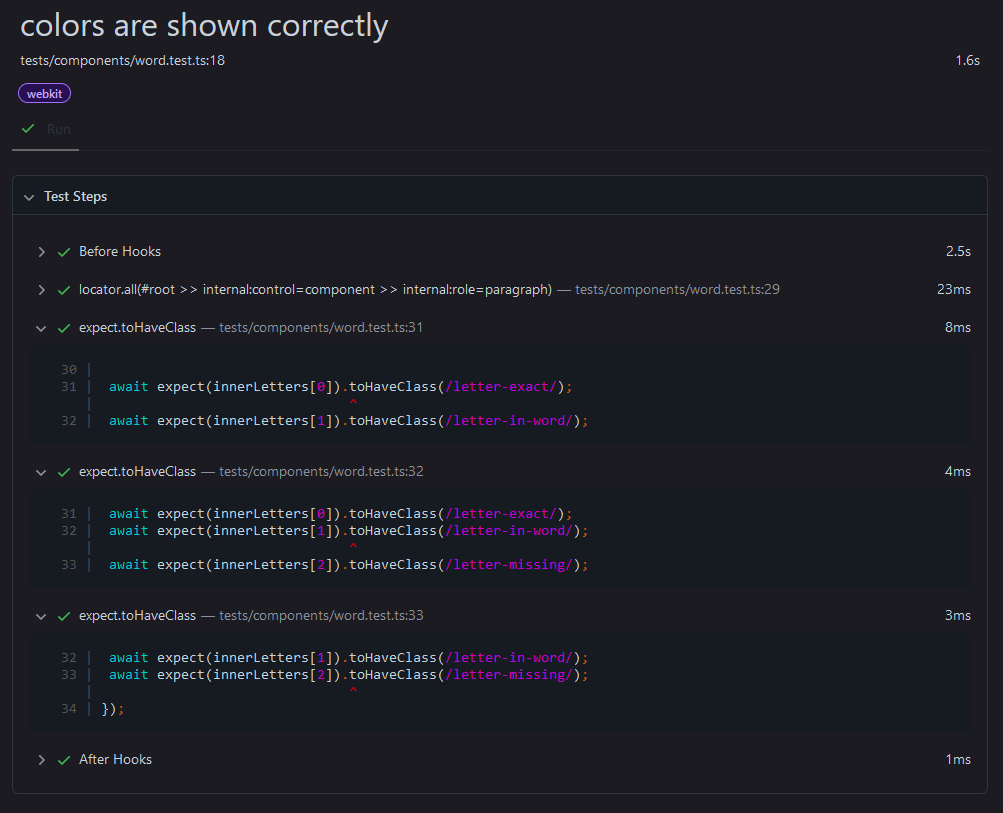
\includegraphics[clip=true, width=\textwidth]{images/tests/playwright_one_test.png}
	\caption{Inspección de un test en Playwright.}
	\label{fig:playwright_test_result}
\end{figure}

\subsubsection{Problemas encontrados}
Playwright puede llegar a ser complejo de instalar según sea el sistema del usuario a ejecutar los tests. Para la realización de este TFG se han dedicado varias horas únicamente a conseguir que Playwright consiga ejecutar los tests en el entorno en el cual se ha realizado esta (WSL 2 - Ubuntu). Al final el problema se soluciono instalando las librerías necesarias manualmente, en lugar de utilizar el instalador automático. Si durante la instalación de las librerías ocurre el sistema operativo no encuentra alguna, sera necesario limpiar la cache de librerías, en mi caso APT tal y como se indica en \cite{playwright_lib_error}.

\subsection{Servidor de Websockets}
Los tests para el servidor de Websockets se han centrado en el testeo unitario de la comprobación de palabras para la generación de resultados Wordle, además se ha comprobado con test unitarios el comportamiento de alguna función de dominio.

Con la flexibilidad de testeo que ofrece Deno, se ha programado un sistema que es capaz de generar tests unitarios para las palabras que se requiera (fragmento de Código \ref{alg:deno_tests}). Para ello, se genera un test con varios steps (pasos), cada step es una nueva palabra para probar, todo ello es posible generando una estructura de datos que almacene el intento del jugador, y el resultado que se debería de obtener tras el intento. Después, tan solo es necesario recorrer la estructura de datos generando los steps (fragmento de Código \ref{alg:deno_tests_2} ).

\begin{mytypescript}[float={!h},caption={Implementación del sistema de creación de test automáticos.},label={alg:deno_tests}]
	const validations: WordTest[] = [
		{ solution: "TESTS", words: [
			{
				word: "TESTS",
				expected: [2, 2, 2, 2, 2],
			},
			{
				word: "TESTT",
				expected: [2, 2, 2, 2, 0],
			},
			{
				word: "SPLIT",
				expected: [1, 0, 0, 0, 1],
			},
			{
				word: "SPLTT",
				expected: [1, 0, 0, 2, 1],
			},
			{
				word: "STLAT",
				expected: [1, 1, 0, 0, 1],
			},
			{
				word: "ATTAT",
				expected: [0, 1, 1, 0, 0],
			},
			{
				word: "AAAAA",
				expected: [0, 0, 0, 0, 0],
			},
			]
		}
	];
\end{mytypescript}

\begin{mytypescript}[float={!h},caption={Implementación del sistema de creación de test automáticos.},label={alg:deno_tests_2}]
	for await (const validation of validations) {
		for await (const word of validation.words) {
			await test.step({
				name: "${validation.solution} -> ${word.word}",
				fn: () => {
					const result = validateWord(word.word, validation.solution);
					assertEquals(result, word.expected);
				},
			});
		}
	}
\end{mytypescript}

Tras ejecutar este test obtenemos los siguientes resultados:

\begin{figure}[H]
	\centering
	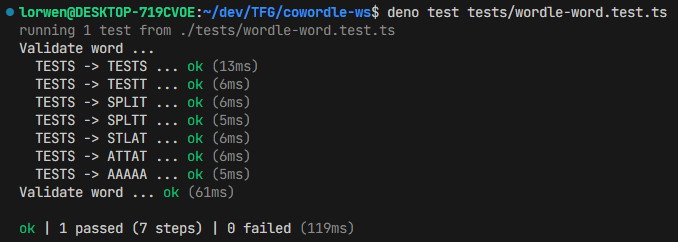
\includegraphics[clip=true, width=0.75\textwidth]{images/tests/deno_test_wordle.png}
	\caption{Resultado del test de validación de palabras.}
	\label{fig:deno_test}
\end{figure}

Como se puede comprobar, siguiendo la estructura de datos, cada step ejecutado ha comprobado si el resultado tras ejecutar la función \textit{validateWord} ha retornado el resultado esperado o no. Además, nos muestra por pantalla todos los intentos que se han realizado.

\subsubsection{Problemas encontrados}
Deno es un entorno para ejecutar Typescript muy reciente y todavía no dispone de todas las mejoras para realizar tests que pueden llegar a ofrecer sistemas más consolidados, como sistemas para hacer mocks, este problema es aliviado por la flexibilidad ofrecida por Javascript, que permite realizar pseudo-mocks de manera manual.

Aun así, la experiencia de testeo con Deno es satisfactoria.

\section{Distribución y despliegue}

Existen varias maneras de ejecutar la aplicación, la opción más sencilla es utilizar Docker, aunque también está disponible de levantar la aplicación desde el código directamente.

\subsection{Utilizando Docker}
Utilizando Docker, podemos levantar la aplicación al completo, tanto la webapp, como el servidor de websockets. Esta es la opción más sencilla y la manera recomendada de levantar la aplicación para su despliegue.

Para levantar la aplicación utilizando Docker necesitamos tener Docker y Docker Compose instalado. Una vez instalado podemos utilizar el siguiente archivo \textit{docker-compose.yaml} (fragmento de Código \ref{alg:docker_compose}). Este archivo indica a Docker que aplicaciones (llamadas servicios) queremos que se ejecuten, aqui podemos agregar aplicaciones propias, o de terceros.

Para desplegar CoWordle, todos las aplicaciones que necesitamos que se ejecuten son propias. La primera es la webapp, y la segunda es el servidor de websockets. Además, en el archivo estamos creando una red entre ambas aplicaciones que permite la comunicación interna de ambas, este paso no es necesario para realizar el despliegue en Okteto, pero si puede llegar a ser necesario en caso de realizar el despliegue en otros sistemas. Las variables de entorno las utiliza 

\begin{mypython}[float={!h},caption={\textit{docker-compose.yaml} para despliegue en Okteto.},label={alg:docker_compose}]
	version: "3.9"
	services:
	webapp:
		image: "lorwen/cowordle-webapp:latest"
		ports:
		- 4173:4173
		networks:
		- inner-network
		environment:
		- PUBLIC_WEBSOCKET_URL=https://websockets-dokest.cloud.okteto.net
		- PUBLIC_WEBSOCKET_EXTERNAL_URL=https://websockets-dokest.cloud.okteto.net
		depends_on:
		- websockets
	websockets:
		image: "lorwen/cowordle-ws:latest"
		ports:
		- 9000:9000
		networks:
		- inner-network
	networks:
		inner-network:
\end{mypython}

Una vez dispongamos de un archivo \textit{docker-compose.yaml}, podemos utilizar el siguiente comando para levantar la aplicación.

\begin{mypython}[float={!h},caption={Comando para levantar todas las aplicaciones utilizando Docker.},label={sh:run_docker}]
	$ docker compose up
\end{mypython}

Si queremos levantar la aplicación en segundo plano, podemos utilizar el siguiente comando en su lugar.

\begin{mypython}[float={!h},caption={Comando para levantar todas las aplicaciones utilizando Docker en segundo plano.},label={sh:run_docker_bg}]
	$ docker compose up -d
\end{mypython}

En la documentación oficial de Docker Compose explican más opciones para utilizar Docker Compose \cite{DockerComposeDocs}, pero con los comandos mostrados anteriormente es suficiente para levantar CoWordle.

Una vez esté levantada la aplicación, podemos utilizar la URL \href{http://localhost:4173/} para entrar en la aplicación desde cualquier navegador.

\subsection{Utilizando Git o GitHub}
También está disponible la opción de levantar la aplicación desde el repositorio de GitHub, para ello será necesario descargar el código de ambas aplicaciones.

La primera opción es la recomendada para personas que no conozcan la tecnología Git. Tan solo es necesario seguir la documentación oficial de GitHub, y descargar el código de ambos repositorios.

\begin{itemize}
	\item La \textbf{Aplicacion web} se encuentra en el repositorio de GitHub \href{https://github.com/Dokest/cowordle-webapp}.
	\item El \textbf{Servidor websockets} se encuentra en el repositorio de GitHub \href{https://github.com/Dokest/cowordle-ws}.
\end{itemize}

También es posible descargar el código utilizando git con los comandos mostrados (\ref{sh:git_clone_repos}):

\begin{mypython}[float={!t},caption={Comandos git para clonar los repositorios.},label={sh:git_clone_repos}]
	$ git clone https://github.com/Dokest/cowordle-ws.git
	$ git clone https://github.com/Dokest/cowordle-webapp.git
\end{mypython}

Una vez descargado el código, tenemos que levantar ambas aplicaciones: para levantar la webapp, será necesario utilizar el comando \ref{sh:run_webapp}.

\begin{mypython}[float={!t},caption={Comando para levantar la webapp.},label={sh:run_webapp}]
	$ npm run dev
\end{mypython}

Para levantar el servidor de websockets, será necesario utilizar el comando \ref{sh:run_ws_server}.

\begin{mypython}[float={!t},caption={Comando para levantar el servidor de Websockets.},label={sh:run_ws_server}]
	$ deno task dev
\end{mypython}

Una vez levantadas ambas aplicaciones, podemos acceder a CoWordle utilizando la URL \href{http://localhost:4173/}{http://localhost:4173/}.
